% \special{dvipdfmx:config z 0}
\documentclass[withoutpreface]{cumcmthesis} %去掉封面与编号页
\title{基于logisim的32位多周期微程序控制MIPSCPU数据通路和微程序控制器设计} %实验名称
\tihao{A}            % 题号
\baominghao{}    % 报名号
\schoolname{安徽大学}
\membera{成员A}
\memberb{成员B}
\memberc{成员C}
\supervisor{}
\yearinput{}     % 年
\monthinput{}      % 月
\dayinput{}        % 日

\begin{document}
\maketitle
\begin{tabular}{cccccc}
\hline
学  号 & E12214052 &专  业 & 计算机科学与技术 &姓  名 & 赵宸宇 \\
\hline
实验日期 & 2024年9月10日 &教师签字 & 徐晨初 &成  绩&\\
\hline
\end{tabular}
\begin{abstract}
本次实验设计和实现一个\textbf{32位多周期微程序控制}的MIPS CPU,为学生深入理解MIPS CPU的设计原理和实现细节提供了良好的实验平台。

\subsection*{该实验的\textbf{主要内容}}
\begin{enumerate}
    \item 实验\textbf{准备}
    \item \textbf{数据通路}设计
    \item \textbf{控制器}设计
    \item 8条指令的\textbf{ISA调通和联调}
    \item 实验\textbf{总结与改进}
\end{enumerate}

\subsection*{该实验的\textbf{主要产出}}
\begin{enumerate}
    \item MarkDown上课\textbf{笔记}和慕课线上\textbf{自学笔记},请见附件
    \item 完整的\textbf{实验报告}材料,包括\textbf{\LaTeX{}文档}和 生成的\textbf{PDF}文档及其附件,请见\textbf{附件和git仓库}
    \item 该实验过程的\textbf{git仓库},包括circ,xlsx等支持材料的变更记录(每期实验延期一周发布);位置:\url{https://gitee.com/cslearnerer/AHU-CSHT}
\end{enumerate}
\end{abstract}


%目录
\tableofcontents


\section{【实验目的】}
\subsection{几大主要任务}
本次实验需要学生完成一个MIPsCPU设计。这CPU是指\textbf{32位MIPsCPU},采用\textbf{多周期微程序}控制机制。具体来说,该设计主要包含以下几个方面:

\begin{enumerate}
\item 首先,\textbf{通过mooc}对实验设计的具体概念\textbf{进行预习},熟悉实验环境。
\item 然后,需要\textbf{设计数据通路},这是该MIPsCPU得以运行的基础框架,也是该后面设计所需要依赖的基础。
\item 再者,需要\textbf{完成控制器的设计}。由于本次实验采用的硬件实现是多周期&微指令的,所以需要先后完成:1.\textbf{指令译码逻辑}; 2.微指令\textbf{存储器}和微程序\textbf{地址转移}逻辑(指令翻译逻辑);3.\textbf{ALU控制}器逻辑。
\item 最后,需要完成的就是\textbf{ISA的调通},所谓ISA的调通和联调就是指本次实验涉及的\textbf{8条指令}的调试成功,以及\verb+sort.hex+\textbf{程序的调试成功}。只有这两个方面都成功了,才能从软件层面说明本次设计的CPU基本可以运行。
\item 作为一个附加项目,再完成CPU的设计工作后,接下来就可以对CPU的设计\textbf{进行完善}。例如\textbf{优化数据通路}的呈现模式、\textbf{优化微指令存储器}的内容设计等等。这些工作大多处于技巧性层面,故而可以通过\textbf{逐步渗透到后面的所有实验中迭代优化工作}。
\item 疑难解答
\end{enumerate}


\section{【实验原理】}
本次实验的实验原理有:

\begin{enumerate}
	\item 首先是\textbf{数字逻辑电路和logisim},数字逻辑电路是本次实验得以进行的关键,是本次实验的底层知识体系。而logisim则负责在软件层面实现&模拟&仿真这个设计。虚拟实验平台logisim为本次实验提供了良好的支持,有利于学生理解实验设计,加速设计。
	\item 然后是\textbf{MIPs32位CPU}的相关内容,包括\textbf{指令集架构、硬件实现、微程序设计等}。对于各个方面,主要的参考内容有百科页面、MIPs指令集手册等等。需要注意的是,MIPsCPU在底层设计和实现上和x86CPU有着很大的不同,例如reg的数量,例如访存的习惯,例如指令的长度和定长特性等。
	\item 最后,就是MIPs指令集下的\textbf{汇编知识},这里主要通过迁移前面所学的MIPs指令集基础知识和x86调试经验来完成这方面的理解和联调运行工作。
	\item 其他方面,还有\textbf{硬布线和微程序控制的区别},这里我选择了后者,这造成的影响将在下文展开谈论。
\end{enumerate}

\section{【实验内容】}
接下来,本文逐步骤讲解实验方案和本次学生完成实验的主要流程。

根据上文【实验目的】提出的实验流程,这里首先需要\textbf{完成数据通路的设计工作}。
\subsection{数据通路设计}
对于\textbf{数据通路},本文参考了HUST提出的MIPsCPU数据通路设计原理图,如下图所示。
\begin{figure}[!htbp]
    \begin{subfigure}[c]{0.4\textwidth}
    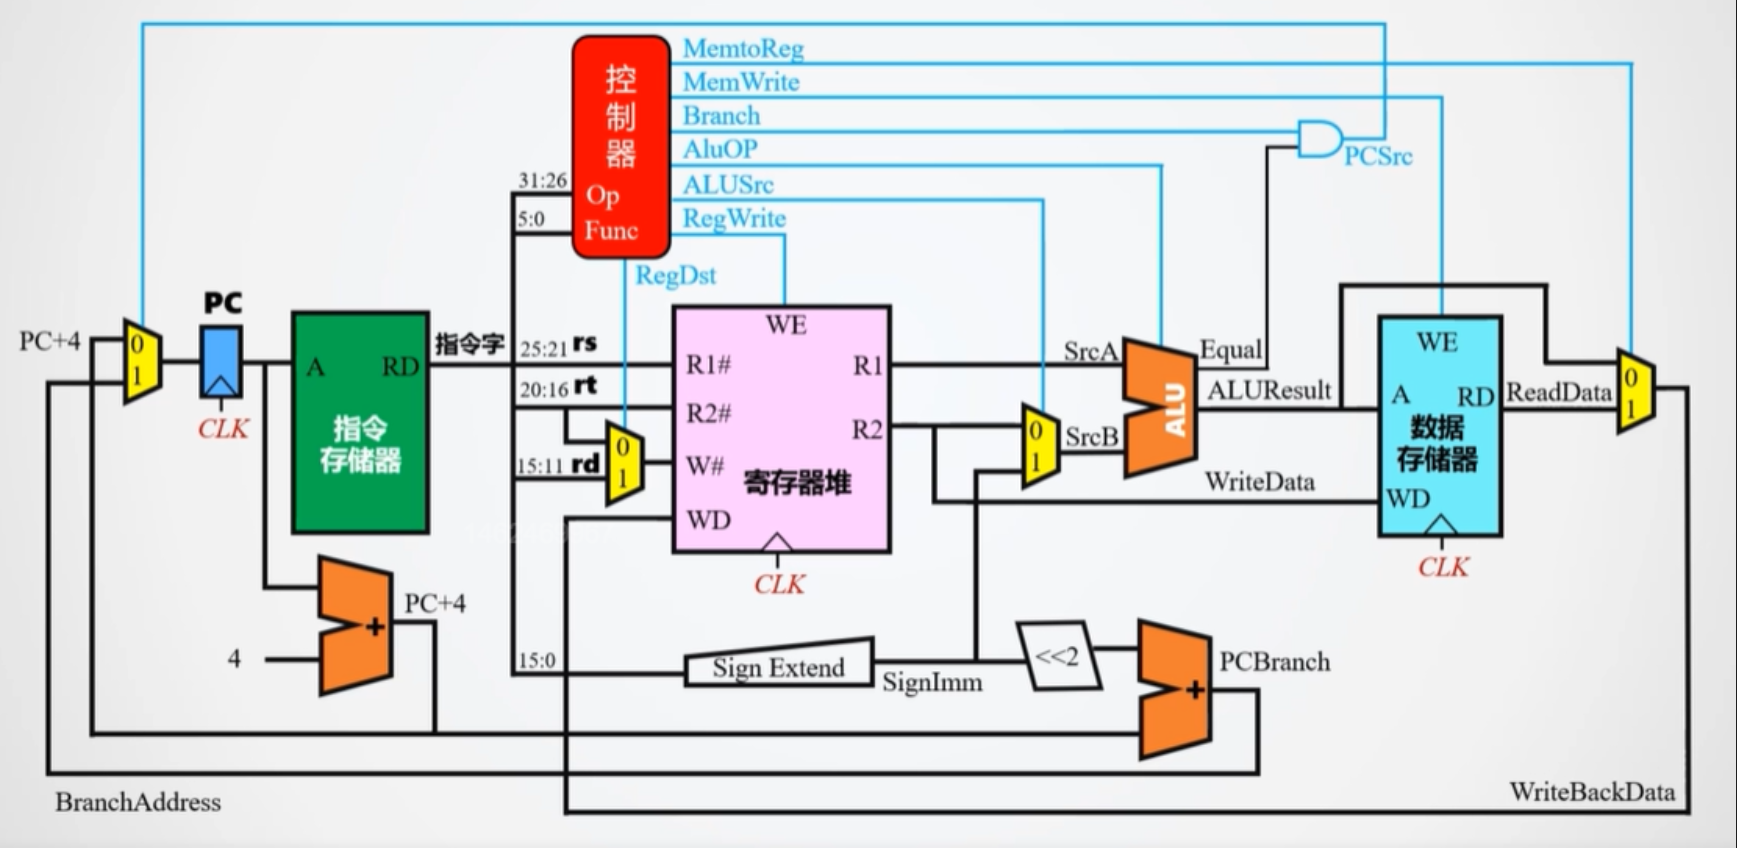
\includegraphics[height=0.12\textheight]{uujutsluuejian}
    \subcaption{数据通路设计原理图}
    \end{subfigure}
    \begin{subfigure}[c]{0.4\textwidth}
    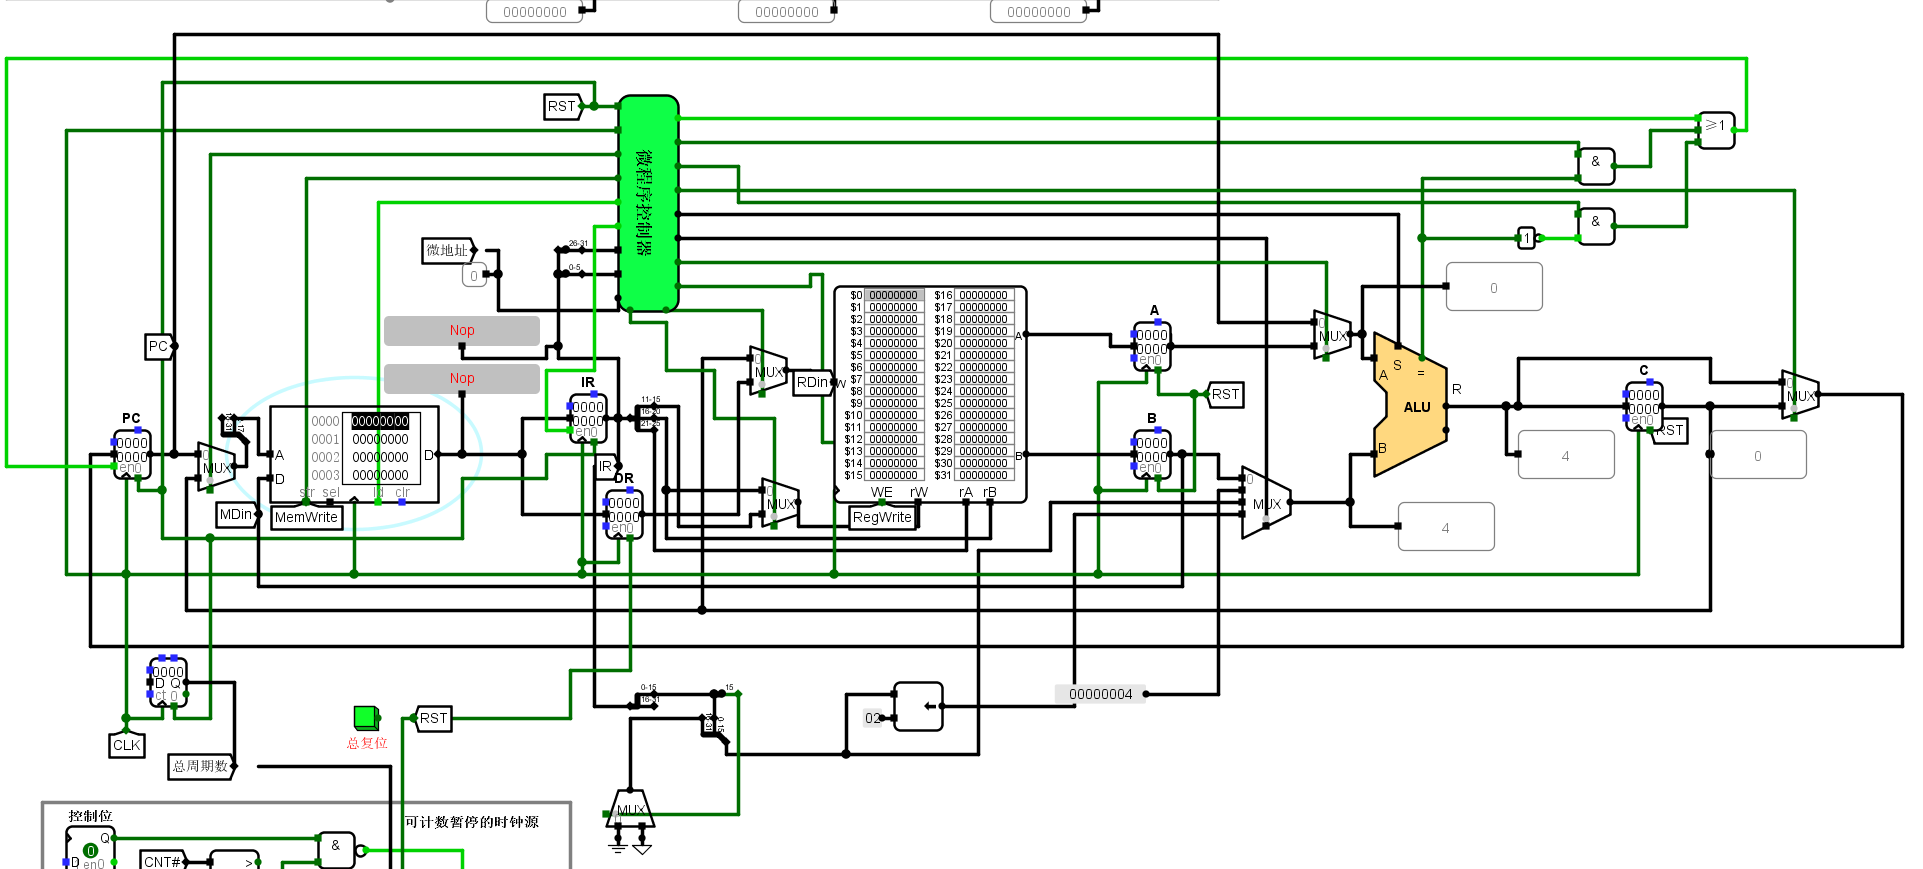
\includegraphics[height=0.12\textheight]{wodeuujutsluuejitu}
    \subcaption{数据通路具体实现}
    \end{subfigure}
    \caption{数据通路}
\end{figure}
对于该原理图,本文参考其设计原理完成了如右图所示的数据通路设计。对于原理图没有提及的如PC位宽等等的问题,本文采用了一定的优化方案来辅助实现。例如,本文的PC采用字节地址存储,当需要使用PC访存时,会有专门电路(PC右侧的分线机构)对PC进行右移操作,同时截断出MM所需的16位地址位宽。

其次,本文对电路细节做了优化,例如:本文使用了cs3410提供的寄存器堆以方便修改和观察CPU运行情况;本文采用了一系列探针机构来显示各个锁存寄存器的内容进而方便调试;本文还对鼠标的操作模式进行了微调,通过将常用按键绑定到鼠标侧键和上下滚轮键,将本地的鼠标进化为了一个logisim专用的调试器。这在之后的调试过程中极大地加速了调试进度。

鉴于是初次实现数据通路,本次实验的数据通路也有不足的地方,其中一个主要点就是:略显凌乱,这将成为今后实验设计技巧渗透中的一大改进方向。
\subsection{控制器的设计}
如下组图所示,本文使用了一种较简单的方式即选择-或门的方式来完成指令译码逻辑和地址转移逻辑的设计工作。
        \begin{figure}[!htbp]
            \centering
            \begin{minipage}[c]{0.4\textwidth}
                \centering
                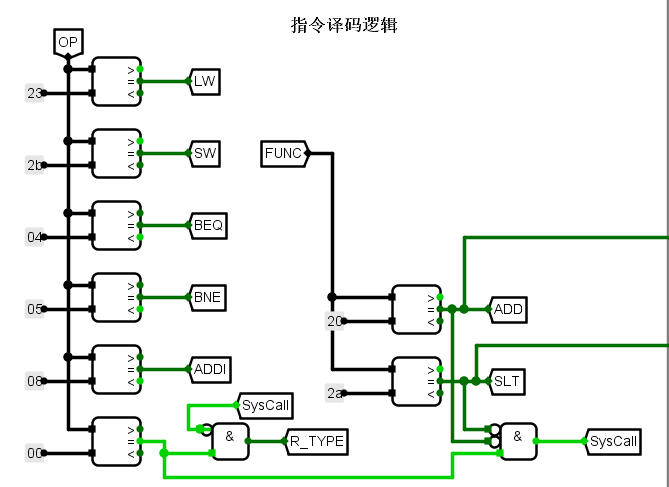
\includegraphics[height=0.12\textheight]{vilkyimaloji}
                \subcaption{指令译码逻辑}
            \end{minipage}
            \begin{minipage}[c]{0.4\textwidth}
                \centering
                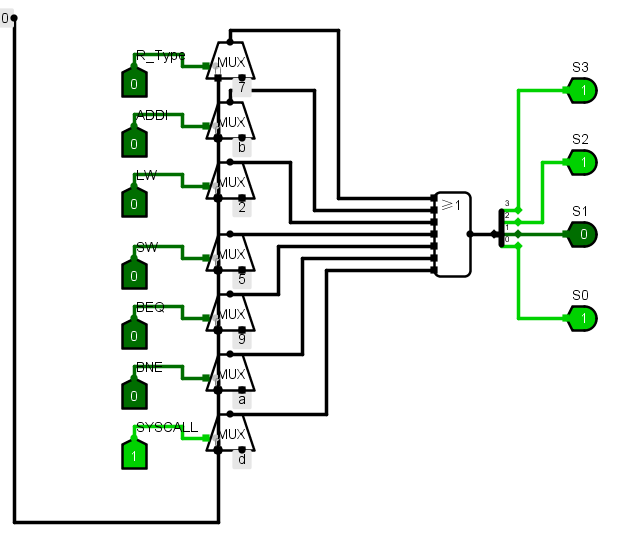
\includegraphics[height=0.12\textheight]{divivryi}
                \subcaption{地址转移逻辑}
            \end{minipage}
            \caption{地址逻辑电路图}
        \end{figure}
其次对于微程序控制器设计,通过设计—联调——设计反复迭代流程,本文得到的目前可以稳定运行的一种设计方案如右图所示。这种设计方案对于微命令的设计参考了HUST提出的设计原理图,如下图所示。
\begin{figure}[!htbp]
    \centering
    \begin{minipage}[c]{0.39\textwidth}
        \centering
        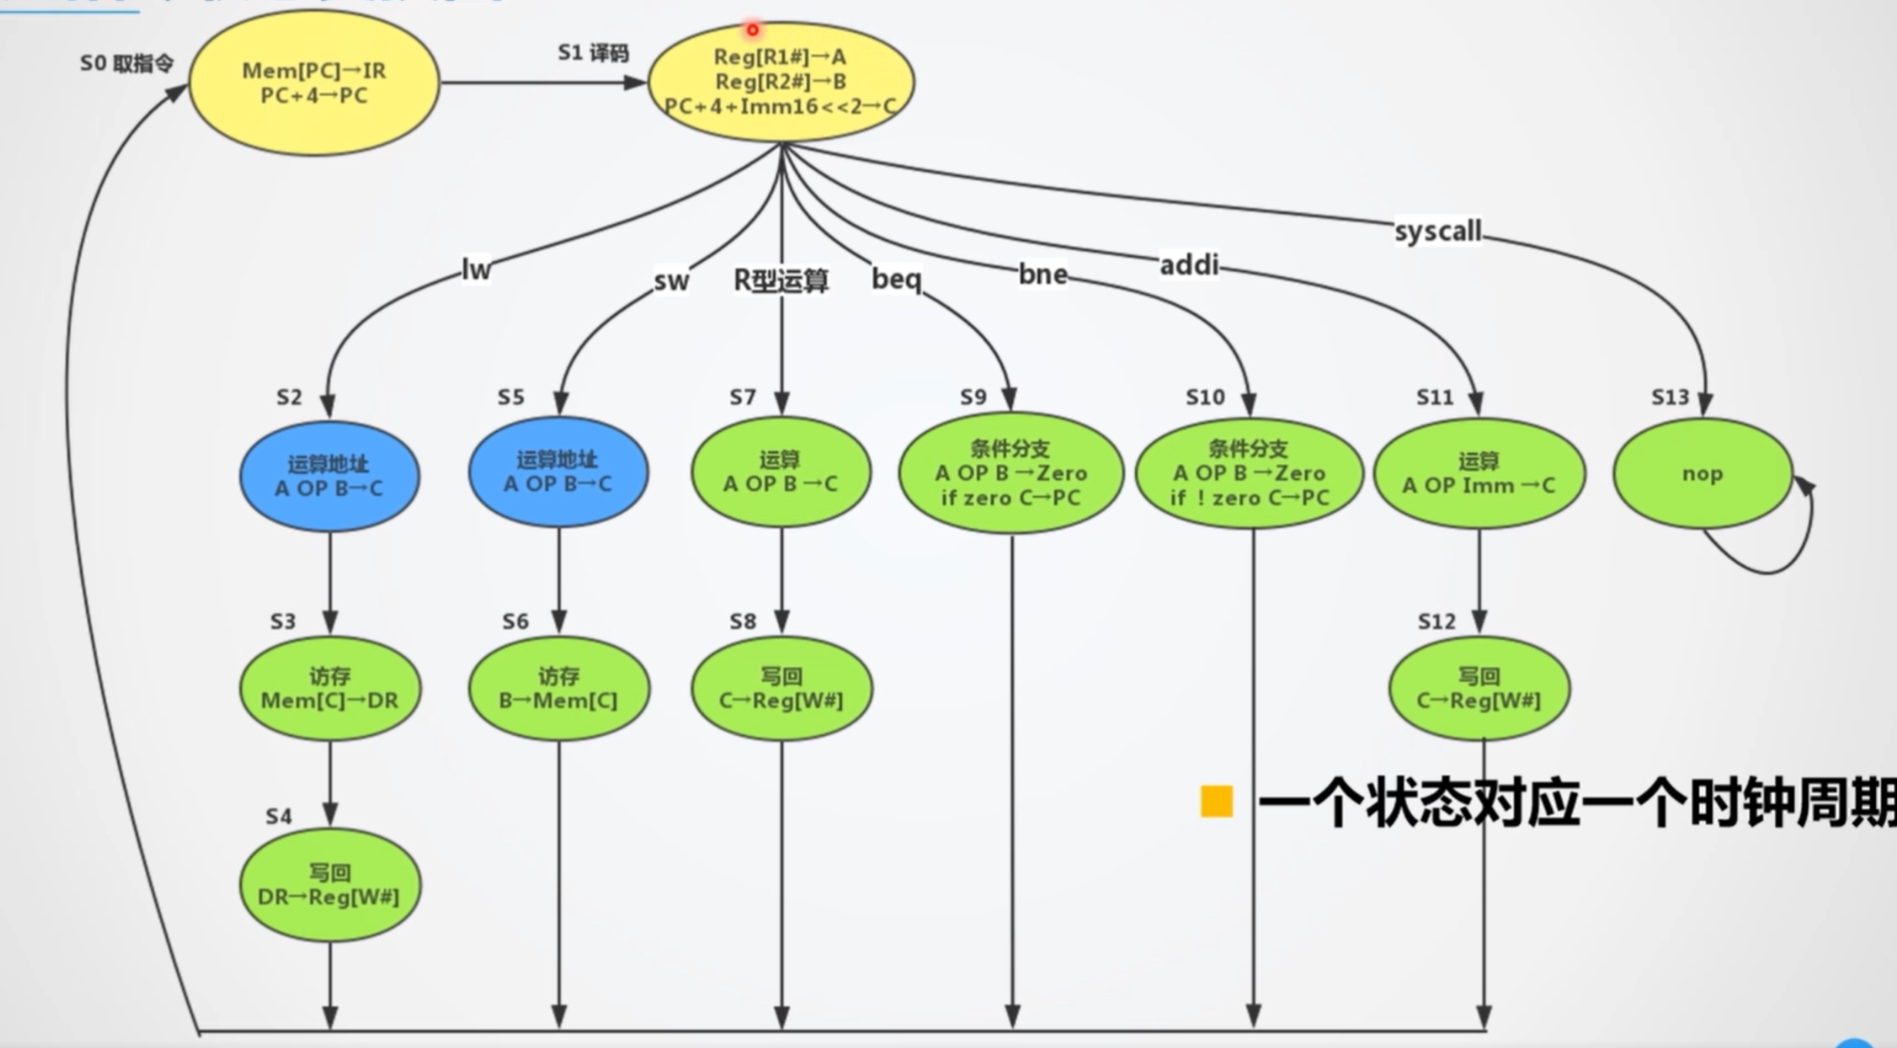
\includegraphics[height=0.12\textheight]{原理图1}
        \subcaption{状态转移图}
    \end{minipage}
    \begin{minipage}[c]{0.39\textwidth}
        \centering
        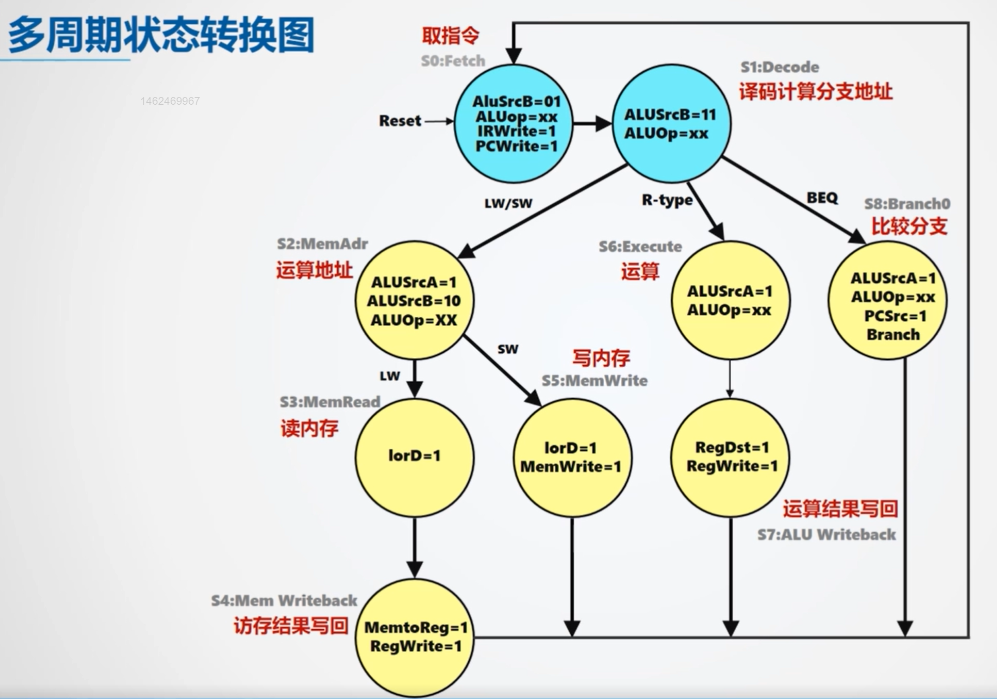
\includegraphics[height=0.12\textheight]{原理图2}
        \subcaption{状态转移—数据通路图}
    \end{minipage}
    \centering
    \begin{minipage}[c]{0.82\textwidth}
        \centering
        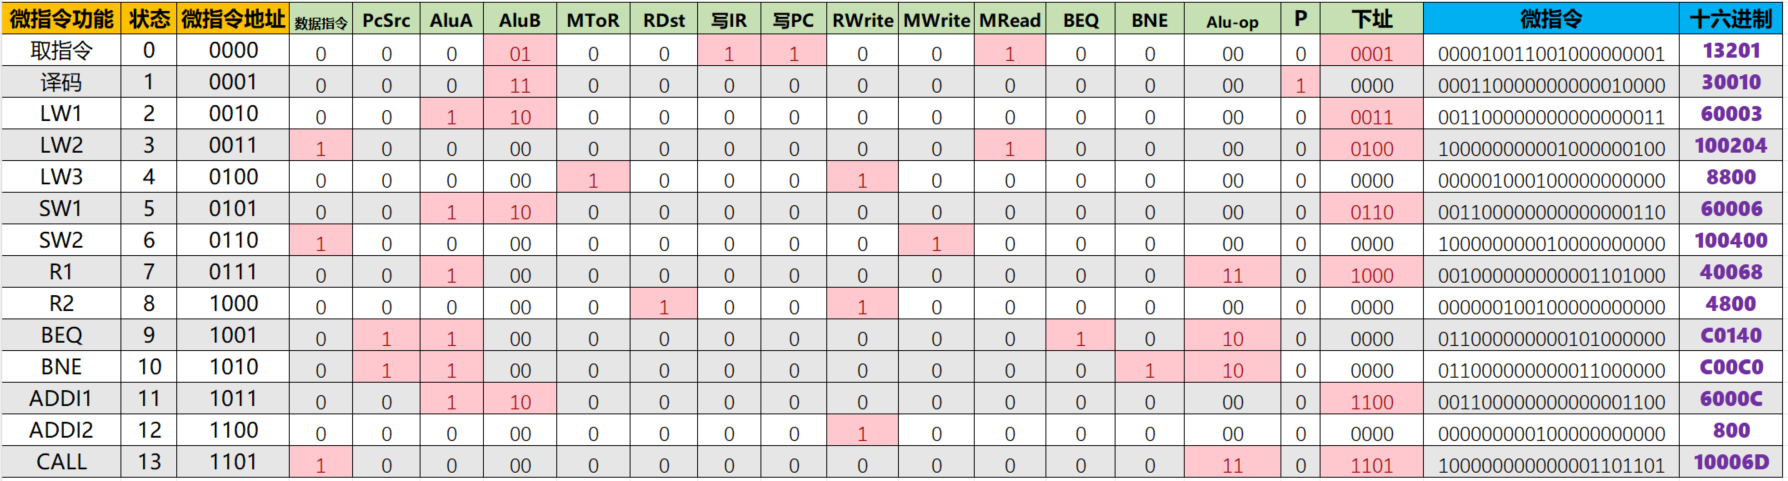
\includegraphics[height=0.12\textheight]{设计方案}
        \subcaption{微命令字段设计案}
    \end{minipage}
    \caption{微程序控制综合设计}
\end{figure}
本文结合此设计原理图,同时还对微程序设计进行了优化。

对于ALU控制逻辑,这里使用选择器配合指令来完成设计工作。鉴于本次所需要实现的指令较少,这才得以使用这一种设计方案,今后在设计大批量指令时,可能需要设计地址转移逻辑那样的专门电路,来优化ALU控制器的设计工作。
\subsection{ISA调通-联调}
最后就是完成8指令调通和sort程序联调。

这里我转回到多周期微程序MIPsCPU的顶层视图。在这里主要用到的操作有:\begin{enumerate}\item 使用总复位软按键和鼠标DPI键(见上文)进行复位和单步调试工作;\item 使用MIPS RAM作为一个接口,将本地LAPTOP上的hex即编译的二进制文件载入其中,即载入汇编程序(机器码);\item 进行单步或多步调试,这里主要是观察两个MIPs反汇编命令窗口、观察当前微指令地址(结合状态转换图)、观察reg堆、观察各个锁存器的探针、使用鼠标上下滚轮切换组件选择和调试模式来修改电路和查看没有探针的二进制内容——通过反复操作以上步骤,即可得知该指令或者说该程序有没有正常运行。进而对电路做进一步修改。\end{enumerate}

具体来说,工作细节如下例所示:
\subsubsection{单指令调通}
例如对一条addi指令,首先需要将addi.hex载入到内存,复位CPU做调试准备。然后需要对照着状态图和addi.asm,结合语义特征,观察addi指令是否按照设计的状态流程 0 - 1 - 11 - 12 -0正确运行。如果在中途发现信号或者数据错误,则需要重视错误发生的地点,这可能是一个锁存器、可能是一个微命令位(即控制器的输出端口的状态没有安装既定方式运行)、也可能是一个reg(这是是rw或w出现了问题)。

总之,通过错误—定位错误—修改错误的调试流程,就可以通过指令的单步调试逐渐发现所有的错误进而将硬件和微程序的根源上的错误通通改正。
\subsection{排序程序调通}
重复以上单指令调试步骤,调试通过后就能确保8条指令均已经正确实现了。

然后直接载入运行sort.hex,即可在RAM中查看得到以下运行结果。如下图所示,-1到6共8个数字均已被正确排序,这标志着本次实验取得圆满成功。
\begin{figure}[!htbp]
    \centering
    \begin{minipage}[c]{0.38\textwidth}
        \centering
        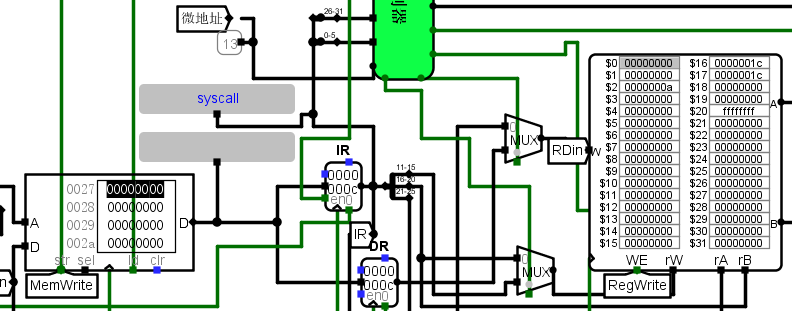
\includegraphics[height=0.12\textheight]{运行结果-电路}
        \subcaption{运行结果-电路}
    \end{minipage}
    \begin{minipage}[c]{0.38\textwidth}
        \centering
        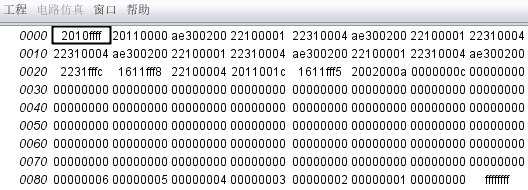
\includegraphics[height=0.12\textheight]{运行结果-数据}
        \subcaption{运行结果-数据}
    \end{minipage}
    \caption{运行结果}
\end{figure}
\subsection{验证}
完成sort排序工作后还应当对实验结果进行验证。经过验证,本次实验到systemcall指令共运行了891个clk,和标称值891一致。

\section{【小结讨论】}
\subsection{疑难解答}
\subsubsection{为什么不能合并LW和SW指令的第三个状态?}
两条指令的第三个状态需要完成的任务相同,所以微命令控制字段是一样的。但是两条指令接下来指令的微命令不一样,所以需要不同的下址字段。

\textbf{故而,不能合并LW和SW指令的第三个状态。}

如果非要合并,则需要增加额外的条件字段以实现不同的微地址转移方式
\subsubsection{多周期时钟周期更长?是否性能更差?}
根据:
\begin{equation}
CLK_{sum}=CPI_{avg}*I_{cnt}
\end{equation}
多周期CPU的CPI更大而指令的总条数不变,因此多周期时钟周期更长。

所以,同样的编译器编译出来的程序,多周期架构的CPU必然使用更多时钟周期。

但是多周期实现的CPU性能不一定就差。

通过使用多周期架构,时钟频率得以提升,因此单一指令的总的运行时间往往可以减少,这导致多周期实现的CPU往往能达到更好的机器性能。
\subsection{小结}
本次实验通过设计和实现一个32位多周期微程序控制的MIPS CPU,使学生深入理解了MIPS CPU的设计原理和实现细节。实验过程中,学生不仅掌握了数据通路和控制器的设计方法,还通过反复调试和优化,提升了对硬件设计和调试的能力。

在数据通路设计方面,我通过合理摆放基础组件,并优化电路细节。完成了数据通路框架的基本设计。

在控制器设计方面,采用了选择-或门的方式完成指令译码逻辑和地址转移逻辑的设计,并通过在后续工作中反复迭代,最终实现了稳定运行的微程序控制器设计。对于ALU控制逻辑,也是和指令译码逻辑的设计相似地,通过选择器配合指令完成了设计工作。

在ISA调通和联调过程中,主要任务是通过单步调试和多步调试,逐步发现并修正硬件和微程序中的潜在错误。在联调成功后最终成功运行了冒泡排序程序,验证了CPU设计的正确性。

总结,本次实验让学生掌握了MIPS CPU的设计和实现方法,在设计的过程中,我感受到了极大的成就感和获得感。通过课前预习,课中设计的实验模式我最终实现了该CPU的设计并对MIPs实现细节、微程序控制器、状态机设计、哈佛架构(学习理论基础时用到的单周期硬布线环境下使用的架构)、冯诺依曼架构(本实验)、硬件-ISA粒度的程序调试有了深刻的理解。这为今后的学习和研究和工作打下了坚实的基础。

\end{document}